\subsection{Timely native service with original full calls}
\label{subsec:native_retention_eval}
Input-confirmed full calls improve timely service while preserving the
original feedback task. On eight previously unused speakers, RevTrace
raises audio coverage meeting both deadlines from 40.6\% to 93.9\% and
whole-run passes from zero to ten of sixteen
(Table~\ref{tab:native_full_confirm}). A paired speaker bootstrap,
keeping both timing repeats together, gives a duration-weighted gain
of 53.3 percentage points (95\% CI [44.8, 59.6]; 20,000 resamples).
All eight source-paired gains are positive, ranging from 27.8 to 61.4
percentage points.
The StreamCorrect adaptation retains
original learned correction and feedback, using fixed 500-ms inputs,
no VAD, and FP32 execution~\cite{vu2026streamcorrect}. Both author-built
policies have two complete workers, the same ASR early-view Consumer and
neural warmup. Conservative execution waits for selected parent feedback;
RevTrace starts conditional full calls and retains them when their
complete inputs are confirmed. This tests complete-call overlap against
waiting for selected parent feedback; core factorization separately tests
computation/view retention.

\begin{table}[t]
\centering
\caption{Complete-call retention on eight previously unused speakers.
Each policy offers 137.864~audio-s, with two fresh trials per speaker.
Coverage is a total; D99 is the median per-run display P99.
Both-board energy is normalized by offered audio.}
\label{tab:native_full_confirm}
\small\setlength{\tabcolsep}{3pt}
\begin{tabular}{@{}lrrrr@{}}
\toprule
Policy & \shortstack{Timely\\coverage (s)} & \shortstack{D99\\(s)} &
\shortstack{Energy\\(J/audio-s)} & Pass\\
\midrule
Conservative & 56.000 & 5.027 & 690.989 & 0/16\\
RevTrace & \textbf{129.460} & \textbf{1.762} & 654.845 & \textbf{10/16}\\
\bottomrule
\end{tabular}
\end{table}

\paragraph{Preserving the original selected task}
Metadata selection froze eight unused AISHELL-1 test speakers
\cite{bu2017aishell} before reference or service inference, with one complete
8--9-s utterance per speaker. Two policies and two fresh repeats give
32 runs with balanced policy order and GPU roles swapped across repeats.
Reference checks and independent actual-Consumer audits bind all 564
selected transitions to complete original inputs/outputs, correction and
returned IDs. Final quality is identical across policies and repeats:
23 edits over 174 unique reference characters (13.22\% CER).
Reference generation is charged separately from service.

\paragraph{Energy over the complete service window}
On the new speakers, RevTrace uses 5.23\% less common-window board energy
than Conservative. The origin-to-physical-drain window includes issued
work that is not used.

\paragraph{Where reusable lookahead runs out}
The six failed trials come from S0901, S0902 and S0915. S0915 contributes
6.996 of the 8.404~uncredited audio-s: both repeats miss the same seven
frontiers from 6~s through EOS. Repeated original corrections refute the
next inputs. Each repeat's six late non-EOS replacements dispatch
2--5~ms after the recorded parent-install event and spend 0.53--0.74~s in
original inference per 0.5-s input. At the 6-s frontier in repeat~0, dispatch is at 7.591~s, the ASR
boundary at 7.976~s, and actual consumption at 8.023~s crosses D2 at
8.000~s. S0901 retains a matching early EOS call after slow preceding
recognition; its ASR boundary still arrives late. S0902 loses lookahead
after full-input refutations. In S0915, repeated refutations exhaust
reusable lookahead as the original inference path outgrows the input cadence.

\paragraph{More selected content meets the deadlines}
Figure~\ref{fig:native_content} separates deadline coverage from content
support. On the eight new speakers, timely coverage whose whole first
view retrospectively matches selected text at that view's own frontier
$G$ rises from 47.000 to 107.162~s (34.1\% to 77.7\% of all offered audio).
No timely coverage has unknown agreement; raw and whitespace-stripped
comparisons agree.
More matching views meet the deadlines under the unchanged selected task.
In the four-speaker resident bank, matching timely coverage rises from
24.0 to 50.259~s.

\begin{figure}[t]
\centering
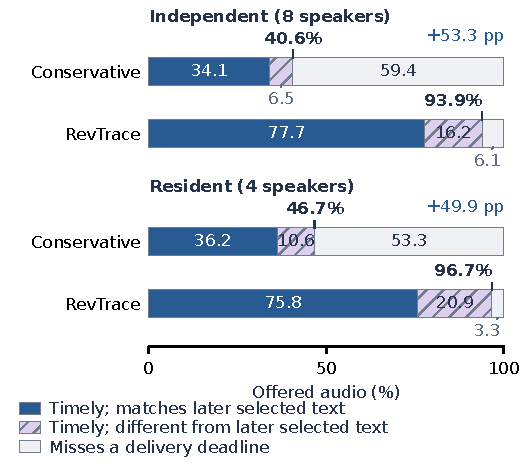
\includegraphics[width=\columnwidth]{figures/native_content.pdf}
\caption{More matching content meets both deadlines: display within 2~s
and certified coverage within 8~s. Independent eight-speaker and resident
four-speaker cohorts offer 137.864 and 66.340~audio-s per policy.
Stacks partition
timely coverage matching later selected whole text at its own frontier,
other timely coverage, and missed deadlines. Retrospective agreement is
distinct from online [SUP] and human accuracy. Boundary labels sum both
timely categories, in rounded percentages.}
\label{fig:native_content}
\end{figure}

\paragraph{Benefits persist across resident requests}
RevTrace raises joint D2/C8 passes from 0/8 to 7/8 requests, and timely
coverage from 31.000 to 64.119 of 66.340~s. Models load once per trial;
both worker PIDs persist across four pre-registered independent requests.
The next request starts only after actual certified consumption of the
previous file EOS. Two policies and two fresh trials preserve all 272
original transitions and each request's own input clock. The second
S0908 repeat is the only failing request, with D99 2.229~s. This single-outstanding closed-loop contract
tests residency.

\paragraph{Benefits are not confined to the D2 cutoff}
In the existing four-speaker banks, we recompute offered-audio coverage over display budgets
from 0.5 to 6~s, keeping every original frontier and EOS tail.
The confirmation budget remains C8.
At 1.5~s, coverage rises from 36.2\% to 84.0\% in matched runs and
from 36.2\% to 78.7\% in resident requests; both policies reach 100\%
at sufficiently loose budgets. At D2, all four speaker-paired gains
are positive in each bank. The advantage spans tighter delivery budgets
and converges as time pressure eases; the original D2/C8 pass rule remains
unchanged.

\paragraph{Input confirmation and view retention}
An earlier 16-run confirmation bank on the four existing sources
has 92 promoted calls whose recognition
begins before selected parent completion; 20 predict successor states
that differ from their original selected results. These observations
separate input eligibility from prediction correctness.

The service gain comes from earlier execution of complete
calls whose inputs are later confirmed. A resident execution separately
exercises view retention: a 5.0-s whole view survives a compatible 4.5-s
selected update with the same tip and job. Its 0.817-s Consumer event-state
holding interval spans that update and ends at legitimate supersession.
Each existing four-speaker RevTrace bank also contains two necessary
incompatible withdrawals.
\par\noindent\textbf{Finding 2: confirmed inputs accelerate the original task.}
Original selection [AU] remains intact when [EL] confirms early full calls;
whole-view retention still requires [SUP] independently.
